\subsection{Tuning of GRASP}
This section is dedicated to the tuning of the probability parameter in the GRASP Variant of the Nearest Neighbour algorithm.

The Greedy Randomized Adaptive Search Procedure (GRASP) is a technique that introduces randomization in the choices of the Greedy Algorithms.
Applied to the Nearest Neighbor algorithm, it actually works by adding a certain probability value \textit{p} that slightly modifies its behavior of improvement of the current solution.

At each iteration, instead of choosing the nearest node to the current one, we have a \textit{p} probability of choosing the second nearest node. That way we can add some randomness to the algorithm and this can actually improve the overall optimality of the final solution.
This variant has been implemented in the project and runs similarly to the multistart Nearest Neighbor algorithm within a time limit, and with different starting nodes at each iteration.

We run the GRASP algorithm multiple times within a certain time limit, each iteration with a different starting node $v \in V$. We tested 5 different probabilities of choosing the second nearest node and the results are shown in Figure \ref{fig:grasp}

\begin{figure}[!h]
    \centering
    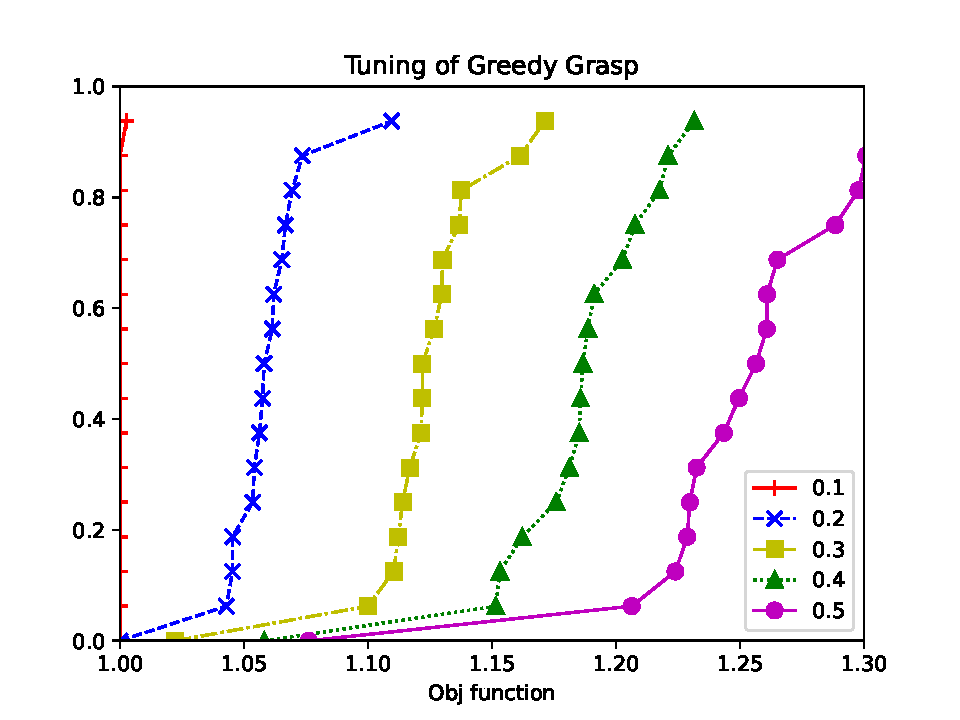
\includegraphics[width=\textwidth]{images/grasp.pdf}
    \caption{Tuning of Probabilities in GRASP}
    \label{fig:grasp}
\end{figure}

As can be seen, the best solution is the one with $p = 0.1$ meaning that we have better results when the algorithm chooses principally the nearest node and not the second nearest one. The hypothesis that the Nearest Neighbor algorithm results in better performance than the GRASP variant is proved later on in the section showing the Performance Profile of all the Heuristic algorithms.


